\section{40GBASE-T}

\subsection{Wprowadzenie}
40GBASE-T jest technologią transmitowania ramek Ethernetowych z prędkością 40 gigabitów na sekundę, wykorzystując skrętkę jako medium. Technologia została zdefiniowana po raz pierwszy jako część standardu IEEE 802.3ba w 2010 roku.

40GBASE-T zapewnia dwukierunkową komunikację przez cztery przewody skrętki. Każdy przewód transmituje ¼ zgromadzonych danych.

\subsection{Położenie 40GBASE-T w modelu OSI}
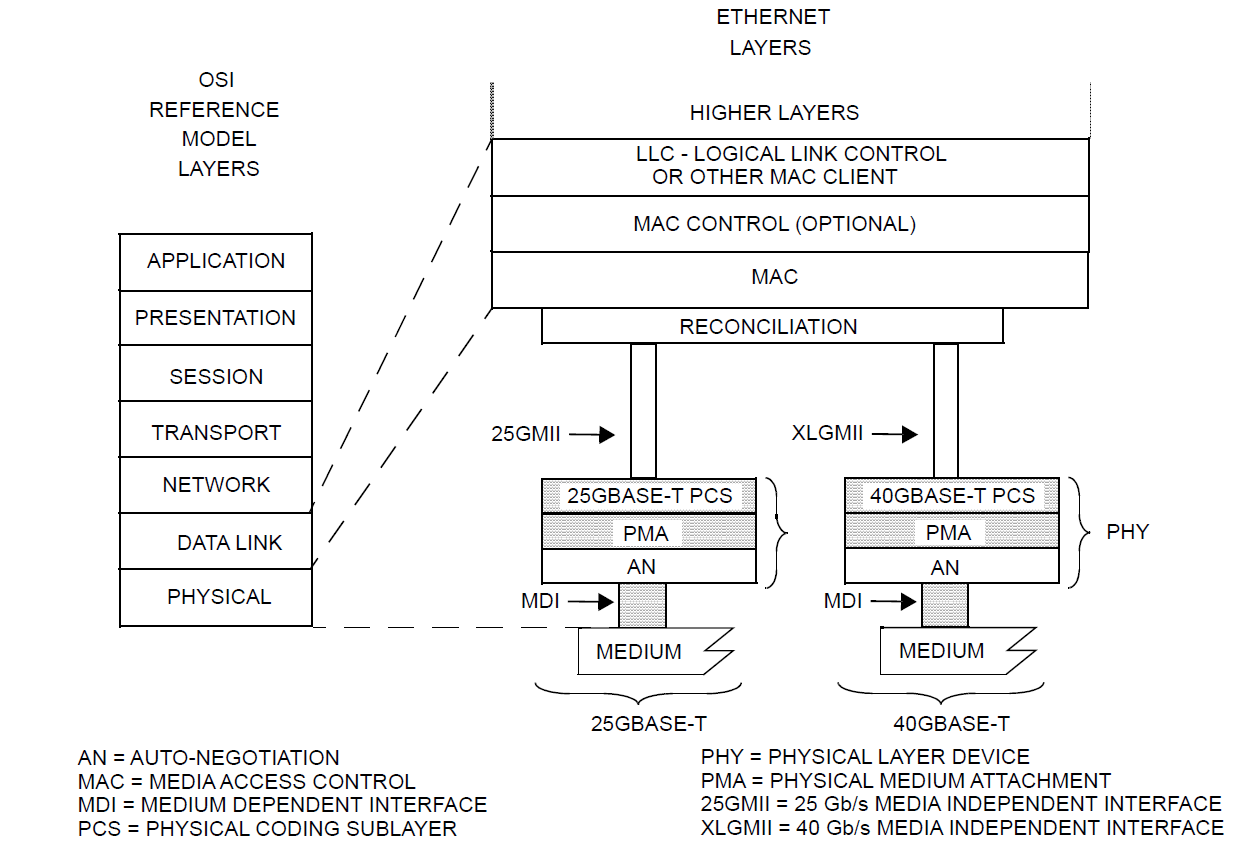
\includegraphics[scale=0.4]{25-40-gbase-osi}

\subsection{Modulacja w 40GBASE-T}
\subsubsection{Wprowadzenie}
Technologia 40GBASE-T wykorzystuje 16-poziomową modulację PAM - mając 16 różnych poziomów amplitudy możemy zakodować 16 różnych wartości co daje nam 4 bity danych.
Oprócz bitów niosących dane, przesyła się również bity pomocnicze (auxiliary bits), przez co w rzeczywistości jeden symbol PAM16 koduje 3,125 bitów informacji.
W ciągu każdej sekundy przesyłanych jest 3200 milionów symboli co przekłada się na prędkość transmisji równą 10 Gb/s (3,125 bit/symbol * 3200 MBd) na każdej z czterech par skrętki, co sumarycznie daje transmisję 40 Gb/s.

\subsubsection{Warstwa PCS}
40GBASE-T PCS (Physical Coding Sublayer) jest warstwą odpowiedzialną m.in. za kodowanie i dekodowanie oraz skramblowanie i deskramblowanie.

PCS pobiera dane od warstwy MAC przez interfejs XLGMII. Jest to tzw. Media-Independent Interface, który powstał po to aby warstwy MAC oraz PHY były niezależne od siebie - pozwala pracę kontrolera MAC z warstwą PHY, bez względu na to jakie medium jest w użyciu.

Dane trafiają z XLGMII do PCS przez wektor TXD<63:0> i gromadzone są w 64-bitowe bloki. Po zebraniu 50 takich bloków, pierwsze 48 z nich transkodowane są w 512-bitowe bloki, a pozostałe są do nich dołączane. Dane są następnie skramblowane i dołączany jest do nich bit pomocniczy (auxiliary bit), po czym dzielone są na dwa zbiory - pierwszy z nich trafia do kodera Reed-Solomona, a drugi jest przetwarzany przez koder LDPC (Low density parity check). Otrzymuje się w ten sposób 512*3 bitów zakodowanych przez RS-FEC oraz 512*4 bitów - LDPC, które łączone są w 7-bitowe grupy u0, u1, u2, c0, c1, c2, c3.


\subsubsection{Mapowanie ramki LDPC na DSQ128}
Zamianę 7-bitów u0, u1, u2, c0, c1, c2, c3 pokazuje poniższy algorytm:

Krok 1:
\begin{align*}
    x_{13} &= \neg u_0 * u_2 \\
    x_{12} &= u_0 \oplus u_2 \\
    x_{11} &= c_0 \\
    x_{10} &= c_0 \oplus c_1 \\
    x_{23} &= (u_1 * u_2) + (u_0 * \neg u_1) \\
    x_{22} &= u_1 \oplus u_2 \\
    x_{21} &= c_2 \\
    x_{20} &= c_2 \oplus c_3
\end{align*}

Krok 2:
\begin{align*}
    x_1 &= 8x_{13} + 4x_{12} + 2x_{11} + x_{10} \\
    x_2 &= 8x_{23} + 4x_{22} + 2x_{21} + x_{20}
\end{align*}

Krok 3:
\begin{align*}
    y_1 &= (x_1 + x_2) \mod 16 \\
    y_2 &= (-x_1 + x_2) \mod 16
\end{align*}

Krok 4:
\begin{align*}
    \text{PAM16}_1 &= 2y_1 - 15 \\
    \text{PAM16}_2 &= 2y_2 - 15
\end{align*}

Otrzymane w ten sposób symbole są transmitowane na odpowiednich parach skrętki:

\begin{table}[h]
    \centering
    \resizebox{\textwidth}{!}{%
    \begin{tabular}{ c | c c c c c c c |}
        \cmidrule{2-8}
        Pair A & PAM16$_1$<0> & PAM16$_2$<0> & PAM16$_1$<4> & PAM16$_2$<4> & \ldots & PAM16$_1$<508> & PAM16$_2$<508> \\
        \cmidrule{2-8}
        Pair A & PAM16$_1$<1> & PAM16$_2$<1> & PAM16$_1$<5> & PAM16$_2$<5> & \ldots & PAM16$_1$<509> & PAM16$_2$<509> \\
        \cmidrule{2-8}
        Pair A & PAM16$_1$<2> & PAM16$_2$<2> & PAM16$_1$<6> & PAM16$_2$<6> & \ldots & PAM16$_1$<510> & PAM16$_2$<510> \\
        \cmidrule{2-8}
        Pair A & PAM16$_1$<3> & PAM16$_2$<3> & PAM16$_1$<7> & PAM16$_2$<7> & \ldots & PAM16$_1$<511> & PAM16$_2$<511> \\
        \cmidrule{2-8}
    \end{tabular}}
\end{table}
